%# -*- coding: utf-8-unix -*-
%%==================================================
%% chapter01.tex for SJTU Master Thesis
%%==================================================

%\bibliographystyle{sjtu2}%[此处用于每章都生产参考文献]
\chapter{AKI算法}
\label{chap:Alg}

为了确定一个子密钥集合$K$的实际密钥信息,我们需要一个算法来计算AKI的值并得到一些可能的实际密钥信息集合。
黄佳琳博士在其博士论文\cite{huang2014revisiting}中提出了一个自动化搜索密钥信息泄露的工具,但该工具设计的算法是一个贪心算法,只能计算出AKI的一个合理上界,无法得到真实的AKI值。
一个AKI的合理上界可以用来进行攻击可能性的分析,但无法用来实际分析一个密钥编排方案的强弱。
Lin等人在\citen{lin2016automatic}中提出了一种对密钥桥技术(Key-Bridging Technique\citen{dunkelman2010improved})的自动化搜索算法,但时间复杂度极高,无法进行大量不同$K$的计算,并且也存在一些反例无法计算(后文中将会提到一个反例)。
因此,现有的AKI算法由于只能给出AKI的一个合理上界,只能用于攻击分析,无法用来分析密钥编排方案的强弱好坏,也不能用来改进密钥编排方案的设计。
本章将会介绍一种全新的基于图论的AKI算法,将会在多项式时间复杂度内计算出真实的AKI值。

\section{单轮加密的AKI}
在介绍完整的AKI算法之前,我们首先从简化版的问题开始考虑——仅有一轮加密时的AKI计算。
我们假设子密钥集合$K$全部集中在第$r$轮上,然后只考虑$r$轮和$r-1$轮两轮之间的依赖关系。
为了解决这个问题,我们将使用图论中二分图的思想来将编排方案、密钥比特、依赖关系等参数量化成图,进而将AKI的计算转化为一个图论的问题。
\begin{defn}[二分图]
    设$G(V,E)$是一个无向图,如果顶点集合$V$可以分割为两个互不相交的子集$A,B$且图中每条边的两个顶点分别属于不同的子集,则称$G$为一个二分图,可记为$G(A,B,E)$。
\end{defn}
\begin{figure}
    \centering
    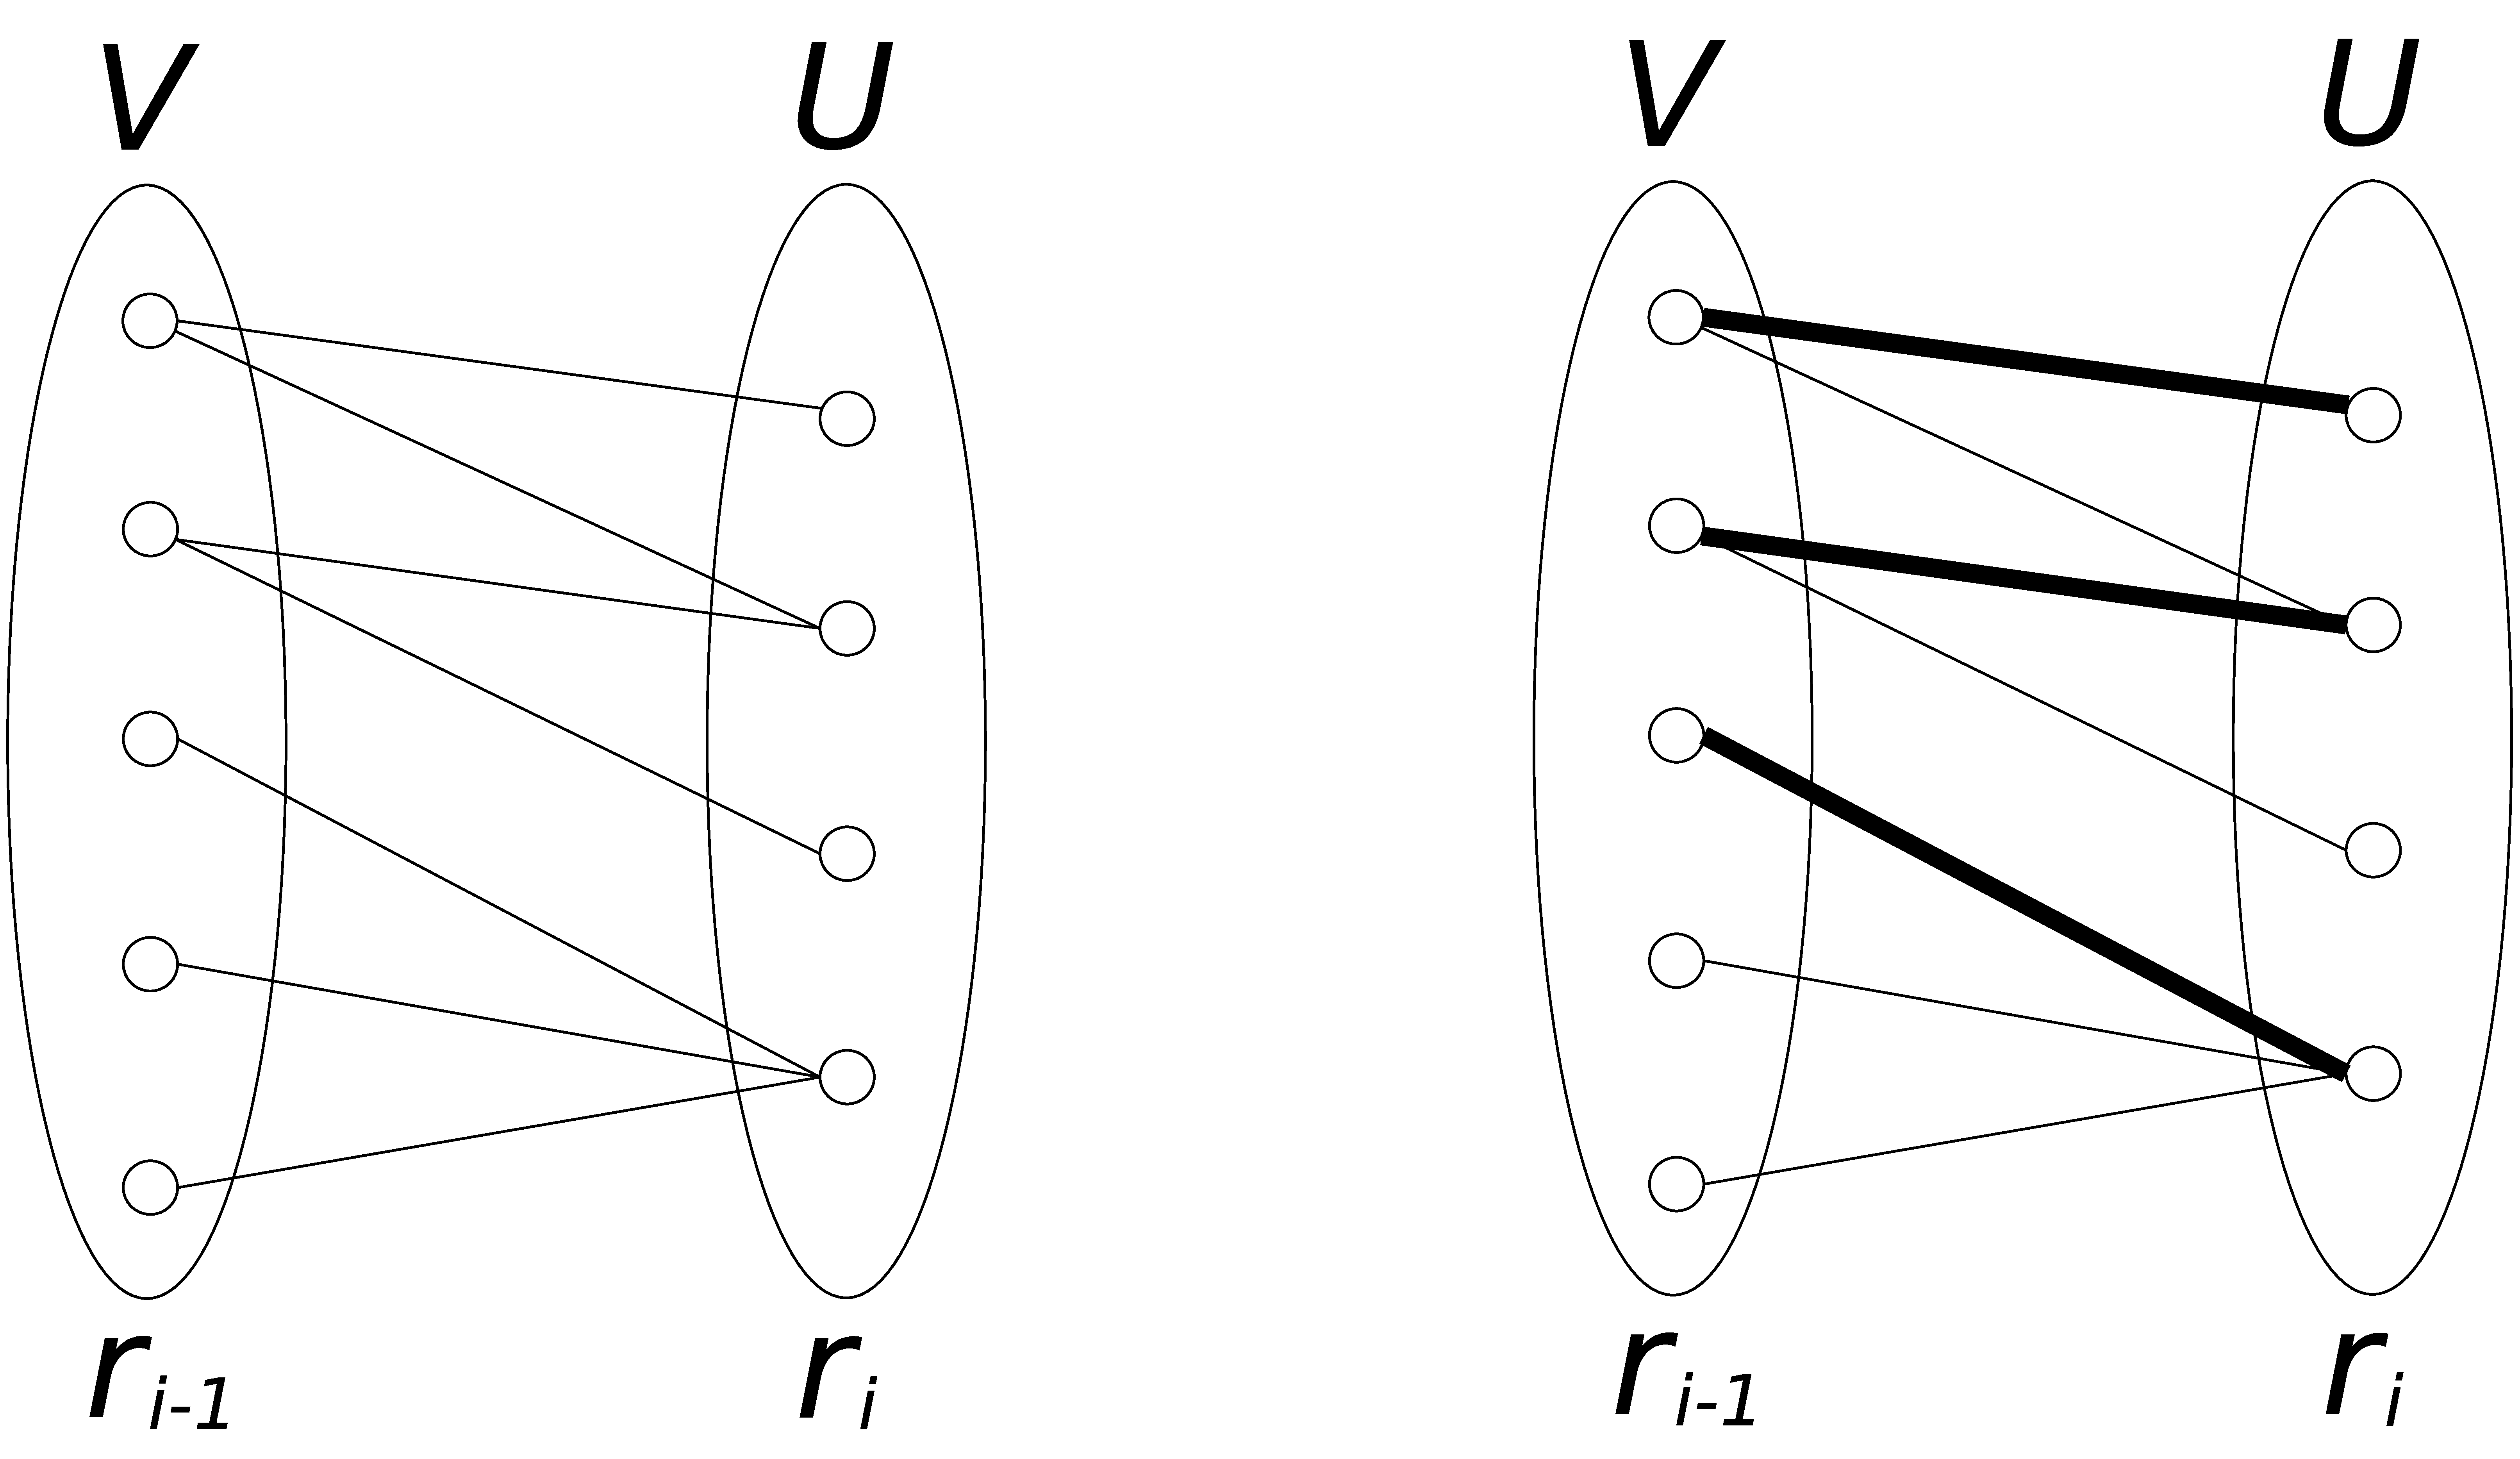
\includegraphics[height=4cm]{bipartite}
    \bicaption[fig:bigraph]{二分图}{一个二分图的例子和它其中一中匹配(被加粗的边)}{Bipartite Graph}{An example of bipartite graph and one of its matching (bold edges)}
\end{figure}
\begin{defn}[图的匹配]
    设$G(V,E)$是一个无向图,如果一个边集$M\subseteq E$中的边两两不相邻(即任意两条边不存在公共的顶点),则成$M$是$G$的一个匹配。
\end{defn}
图\ref{fig:bigraph}中的例子$G(U,V,E)$是一个典型的二分图。我们可以看到所有的边都横跨在两个点集$U,V$之间,而点集的内部不存在任何的边。
在二分图理论中最著名的问题莫过于“二分图最大匹配”问题\citen{west2001introduction},其旨在二分图$G(U,V,E)$中寻找一个最大的匹配$M$。
为了计算最大匹配的值$|M|$,我们需要引入组合数学中著名的霍尔定理\citen{hall1935representatives}的一个拓展:
\begin{thm}[霍尔定理\cite{hall1935representatives}的一个拓展]
    在一个二分图$G(U,V,E)$中,取$U$中的一个子集$X\subseteq U$,记$\Gamma(X)$为$X$的“邻居”,即所有$V$中与$X$中点相邻的点的集合。
    令$\delta(U)=max_{X\subseteq U}\{|X|-|\Gamma(X)|\}$,则有:
    $$MaxMatching(G)=|U|-\delta(U)$$
    \label{thm:hall}
\end{thm}
为了建立轮AKI问题与二分图之间的关系,我们需要这样思考:$r-1$轮和$r$轮的子密钥分别对应子集$V$和$U$中的一个顶点,而这两轮比特之间的一条依赖关系对应横跨$U,V$之间的一条边。
对于给定的子密钥集合$K$(均在$r$轮上),我们把$K$中所有的比特转化成顶点集合$U$,将$K$所依赖的所有$r-1$轮的比特转化为顶点集合$V$,他们之间的依赖关系转化为边集$E$,这样就可以构造出一张二分图$G(U,V,E)$。
这样构造之后,我们重新考虑定理\ref{thm:hall}中的子集$X$(可以视为$K$的一个子比特集合),它的“邻居”$\Gamma(X)$实际上包含了$X$依赖的所有$r-1$轮上的比特,即用$\Gamma(X)$中的所有比特可以推出$X$中的所有比特。
因此,我们可以得出以下引理:
\begin{lem}
    给定一个集中在一轮上的子密钥集合$K$和它的一个子集$X$,令$K'=\Gamma(X)\cup(K\backslash X)$,则$K'$是$K$的一个密钥信息集合。
\end{lem}
\begin{proof}
    由于$\Gamma(X)$可以推出$X$,而$K\backslash X$显然可以推出$K\backslash X$本身,则$K'$可以推出$K$,因此$K'$是$K$的一个密钥信息集合。
\end{proof}
为了找出$K$的实际密钥信息集合,我们需要找到一个最小的密钥信息集合。由于
$$|K'|=|K|-|X|+|\Gamma(X)|=|K|-(|X|-|\Gamma(X)|)$$
又由前文构造出的图$G(U,V,E)$,我们可以得到实际密钥信息集合$K'_{min}$必然满足:
\[
\begin{split}
    |K'_{min}|&=min\{|K|-|X|+|\Gamma(X)|\}\\
              &=|U|-max_{X\subseteq U}\{|X|-|\Gamma(X)|\}\\
              &=|U|-\delta(U)=MaxMatching(G) \qquad\ref{thm:hall}
\end{split}
\]
因此,一个子密钥集合$K$的实际密钥信息的值等于由$U=K$构造出的二分图$G(U,V,E)$的最大匹配的值,且实际密钥信息集合为$K'_{min}=\Gamma(X_{max})\cup(K\backslash X_{max})$,其中$X_{max}$是使$|X|-|\Gamma(X)|$最大的$X$。

\section{AKI-最小割算法}
aaaaa
